\documentclass{report}
\usepackage{graphicx, tikz-cd, float} % Required for inserting images
\usepackage{amsmath, amssymb, amsthm, amsfonts, siunitx, physics, gensymb}
\AtBeginDocument{\RenewCommandCopy\qty\SI}
\usepackage[version=4]{mhchem}
\usepackage[most,many,breakable]{tcolorbox}
\usepackage{xcolor, fancyhdr, varwidth}
\usepackage[Conny]{fncychap}
%Options: Sonny, Lenny, Glenn, Conny, Rejne, Bjarne, Bjornstrup
\usepackage{hyperref, cleveref}
\usepackage{icomma, enumitem} %comma as decimal and continue enumerate with [resume]
%%%%%%%%%%%%%%%%%%%%%%%%%%%%%%
% SELF MADE COLORS
%%%%%%%%%%%%%%%%%%%%%%%%%%%%%%
\definecolor{myg}{RGB}{56, 140, 70}
\definecolor{myb}{RGB}{45, 111, 177}
\definecolor{myr}{RGB}{199, 68, 64}
\definecolor{mytheorembg}{HTML}{F2F2F9}
\definecolor{mytheoremfr}{HTML}{00007B}
\definecolor{mylenmabg}{HTML}{FFFAF8}
\definecolor{mylenmafr}{HTML}{983b0f}
\definecolor{mypropbg}{HTML}{f2fbfc}
\definecolor{mypropfr}{HTML}{191971}
\definecolor{myexamplebg}{HTML}{F2FBF8}
\definecolor{myexamplefr}{HTML}{88D6D1}
\definecolor{myexampleti}{HTML}{2A7F7F}
\definecolor{mydefinitbg}{HTML}{E5E5FF}
\definecolor{mydefinitfr}{HTML}{3F3FA3}
\definecolor{notesgreen}{RGB}{0,162,0}
\definecolor{myp}{RGB}{197, 92, 212}
\definecolor{mygr}{HTML}{2C3338}
\definecolor{myred}{RGB}{127,0,0}
\definecolor{myyellow}{RGB}{169,121,69}
\definecolor{myexercisebg}{HTML}{F2FBF8}
\definecolor{myexercisefg}{HTML}{88D6D1}
%%%%%%%%%%%%%%%%%%%%%%%%%%%%%%%%%%%%%%%%%%%%%%%%%%%%%%%%%%%%%%%%%%%%%%
% Box environments for theorems and problems
%%%%%%%%%%%%%%%%%%%%%%%%%%%%%%%%%%%%%%%%%%%%%%%%%%%%%%%%%%%%%%%%%%%%%
\setlength{\parindent}{1cm}
%================================
% Question BOX
%================================
\makeatletter
\newtcbtheorem{question}{Opgave}{enhanced,
	breakable,
	colback=white,
	colframe=myb!80!black,
	attach boxed title to top left={yshift*=-\tcboxedtitleheight},
	fonttitle=\bfseries,
	title={#2},
	boxed title size=title,
	boxed title style={%
			sharp corners,
			rounded corners=northwest,
			colback=tcbcolframe,
			boxrule=0pt,
		},
	underlay boxed title={%
			\path[fill=tcbcolframe] (title.south west)--(title.south east)
			to[out=0, in=180] ([xshift=5mm]title.east)--
			(title.center-|frame.east)
			[rounded corners=\kvtcb@arc] |-
			(frame.north) -| cycle;
		},
	#1
}{def}
\makeatother
%================================
% DEFINITION BOX
%================================

\newtcbtheorem[]{Definition}{Definition}{enhanced,
	before skip=2mm,after skip=2mm, colback=red!5,colframe=red!80!black,boxrule=0.5mm,
	attach boxed title to top left={xshift=1cm,yshift*=1mm-\tcboxedtitleheight}, varwidth boxed title*=-3cm,
	boxed title style={frame code={
					\path[fill=tcbcolback]
					([yshift=-1mm,xshift=-1mm]frame.north west)
					arc[start angle=0,end angle=180,radius=1mm]
					([yshift=-1mm,xshift=1mm]frame.north east)
					arc[start angle=180,end angle=0,radius=1mm];
					\path[left color=tcbcolback!60!black,right color=tcbcolback!60!black,
						middle color=tcbcolback!80!black]
					([xshift=-2mm]frame.north west) -- ([xshift=2mm]frame.north east)
					[rounded corners=1mm]-- ([xshift=1mm,yshift=-1mm]frame.north east)
					-- (frame.south east) -- (frame.south west)
					-- ([xshift=-1mm,yshift=-1mm]frame.north west)
					[sharp corners]-- cycle;
				},interior engine=empty,
		},
	fonttitle=\bfseries,
	title={#2},#1}{def}
\newtcbtheorem[]{definition}{Definition}{enhanced,
	before skip=2mm,after skip=2mm, colback=red!5,colframe=red!80!black,boxrule=0.5mm,
	attach boxed title to top left={xshift=1cm,yshift*=1mm-\tcboxedtitleheight}, varwidth boxed title*=-3cm,
	boxed title style={frame code={
					\path[fill=tcbcolback]
					([yshift=-1mm,xshift=-1mm]frame.north west)
					arc[start angle=0,end angle=180,radius=1mm]
					([yshift=-1mm,xshift=1mm]frame.north east)
					arc[start angle=180,end angle=0,radius=1mm];
					\path[left color=tcbcolback!60!black,right color=tcbcolback!60!black,
						middle color=tcbcolback!80!black]
					([xshift=-2mm]frame.north west) -- ([xshift=2mm]frame.north east)
					[rounded corners=1mm]-- ([xshift=1mm,yshift=-1mm]frame.north east)
					-- (frame.south east) -- (frame.south west)
					-- ([xshift=-1mm,yshift=-1mm]frame.north west)
					[sharp corners]-- cycle;
				},interior engine=empty,
		},
	fonttitle=\bfseries,
	title={#2},#1}{def}

\newtcbtheorem{theo}%
    {Theorem}{}{theorem}
\newtcolorbox{prob}[1]{colback=red!5!white,colframe=red!50!black,fonttitle=\bfseries,title={#1}}
%================================
% NOTE BOX
%================================

\usetikzlibrary{arrows,calc,shadows.blur}
\tcbuselibrary{skins}
\newtcolorbox{note}[1][]{%
	enhanced jigsaw,
	colback=gray!20!white,%
	colframe=gray!80!black,
	size=small,
	boxrule=1pt,
	title=\textbf{Note:},
	halign title=flush center,
	coltitle=black,
	breakable,
	drop shadow=black!50!white,
	attach boxed title to top left={xshift=1cm,yshift=-\tcboxedtitleheight/2,yshifttext=-\tcboxedtitleheight/2},
	minipage boxed title=1.5cm,
	boxed title style={%
			colback=white,
			size=fbox,
			boxrule=1pt,
			boxsep=2pt,
			underlay={%
					\coordinate (dotA) at ($(interior.west) + (-0.5pt,0)$);
					\coordinate (dotB) at ($(interior.east) + (0.5pt,0)$);
					\begin{scope}
						\clip (interior.north west) rectangle ([xshift=3ex]interior.east);
						\filldraw [white, blur shadow={shadow opacity=60, shadow yshift=-.75ex}, rounded corners=2pt] (interior.north west) rectangle (interior.south east);
					\end{scope}
					\begin{scope}[gray!80!black]
						\fill (dotA) circle (2pt);
						\fill (dotB) circle (2pt);
					\end{scope}
				},
		},
	#1,
}

%%%%%%%%%%%%%%%%%%%%%%%%%%%%%%%%%%%%%%%%%%%%%%%%%%%%%%%%%%%%%%%%%
% SELF MADE COMMANDS
%%%%%%%%%%%%%%%%%%%%%%%%%%%%%%
\newcommand{\sol}{\setlength{\parindent}{0cm}\textbf{\textit{Løsning:}}\setlength{\parindent}{1cm}}
%%%%%%%%%%%%%%%%%%%%%%%%%%%%%%%%%
\usepackage[tmargin=2cm,rmargin=1in,lmargin=1in,margin=0.85in,bmargin=2cm,footskip=.2in]{geometry}\pagestyle{fancy}
\lhead{Minrui Kevin Zhou 2.b}
\rhead{Matematikaflevering 15}

\title{Opgavesæt 2\\
{\Large \textbf{2.b Kemi B}}}
\author{Kevin Zhou}
\date{Oktober 2023}

\begin{document}
\maketitle
\chapter*{Organisk Kemi}
\begin{note}
  Der er \emph{ikke} taget højde for spejlbilledisomeri i følgende løsninger på opgaverne.
\end{note}
\section*{Opgave 2.13}
\sol \\ 
\textbf{a.} I \cref{fig:1} ses reaktionsskemaet for additionsreaktionen. Det skal dog bemærkes, at der her kan forekomme \textit{cis-trans}-isomeri.
\begin{figure}[h]
\begin{center}
  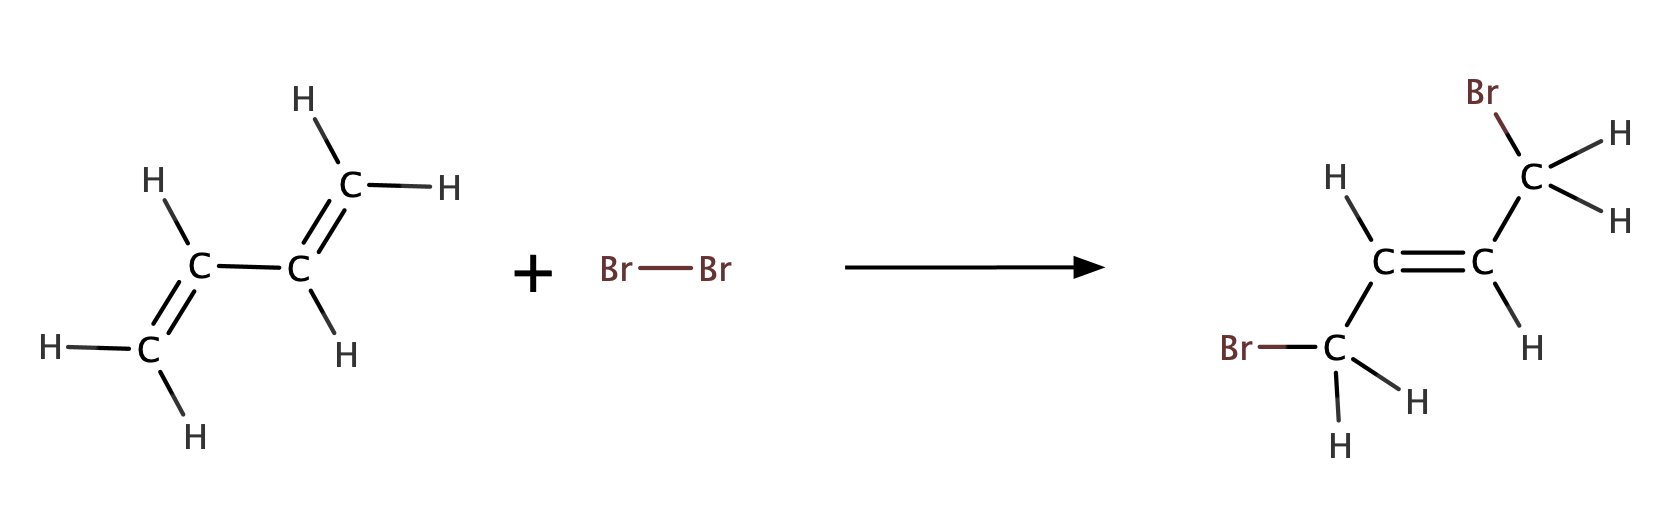
\includegraphics[scale=0.5]{O2_1.png}
\end{center}
\caption{Reaktionsskema lavet vha. MarvinSketch}
\label{fig:1}
\end{figure} \\
\textbf{b.} Navnet på reaktionsproduktet må da være 1,4-dibrombut-2-en. Det skal dog bemærkes, at der her kan forekomme \textit{cis-trans}-isomeri. \\[1ex]
\textbf{c.} Strukturformlen for det dannede stof kan ses i \cref{fig:2}.
Dette stof kaldes for tetrabrombutan.
\begin{figure}[h]
\begin{center}
  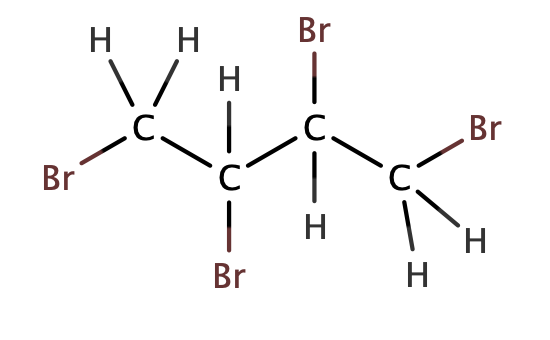
\includegraphics[scale=0.5]{O2_2.png}
\end{center}
\caption{Strukturformlen for tetrabrombutan}
\label{fig:2}
\end{figure}\\ 
\textbf{d.} Vi starter med at beregne stofmængden af buta-1,3-dien.
\begin{equation*}
\begin{split}
  n(\ce{C4H6})&=\frac{m(\ce{C4H6})}{M(\ce{C4H6})}\\ 
  &= \frac{8,50 \;\unit{g} }{54,09\;\unit{g/mol} }\\ 
  &= 0,157145498\;\unit{mol} 
\end{split}
\end{equation*}
Stofmængdeforholdet mellem buta-1,3-dien og dibrom er 1:2. Dette kan bekræftes ved opskrivning af reaktionsskemaer, der dog er udeladt i denne opgave. Altså må følgende gælde.
\begin{equation*}
\begin{split}
  m(\ce{Br2}) &= M(\ce{Br2}) \cdot n(\ce{Br2})\\ 
  &= 159,81 \;\unit{g/mol} \cdot 2 \cdot n(\ce{C4H6})\\ 
  &\approx 50,2 \;\unit{g} 
\end{split}
\end{equation*}
Altså vil massen af den mængde dibrom, der skal anvendes til fuldstændig bromering af $8,5 \;\unit{g} $ buta-1,3-dien være $50,2 \;\unit{g} $.

\section*{Opgave 2.14}
\sol \\ 
\textbf{a.} Reaktionsskemaet ses i \cref{fig:3}, hvor reaktionsprodukterne hedder henholdsvis 2-chlor-2-methylbutan og hydrogenchlorid.
\begin{figure}[H]
\begin{center}
  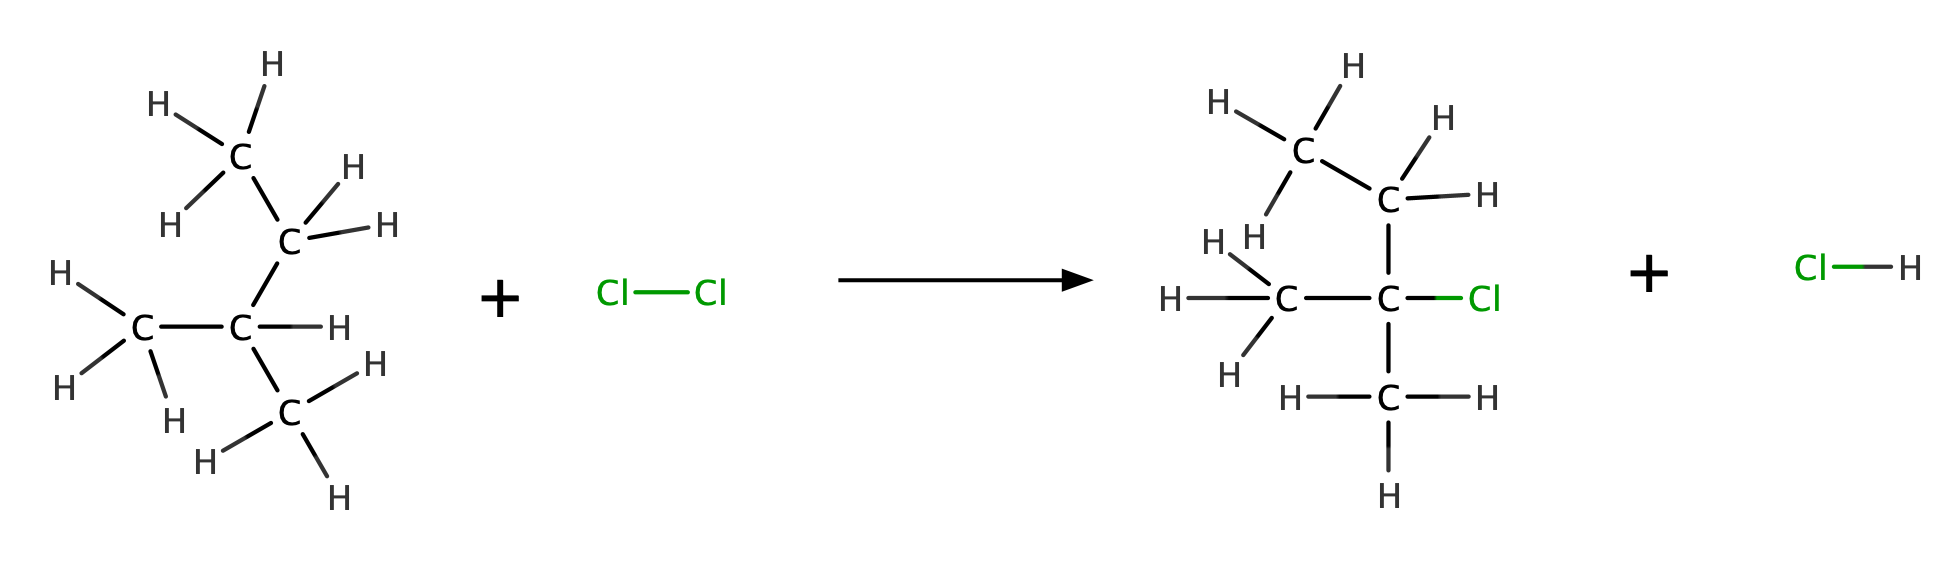
\includegraphics[scale=0.5]{O2_3.png}
\end{center}
\caption{Reaktionsskema lavet vha. MarvinSketch}
\label{fig:3}
\end{figure} 
\textbf{b.} Reaktionsskemaet ses i \cref{fig:4}, hvor reaktionsprodukterne hedder henholdsvis 2,3-dichlor-2-methylbutan og hydrogenchlorid.
\begin{figure}[H]
\begin{center}
  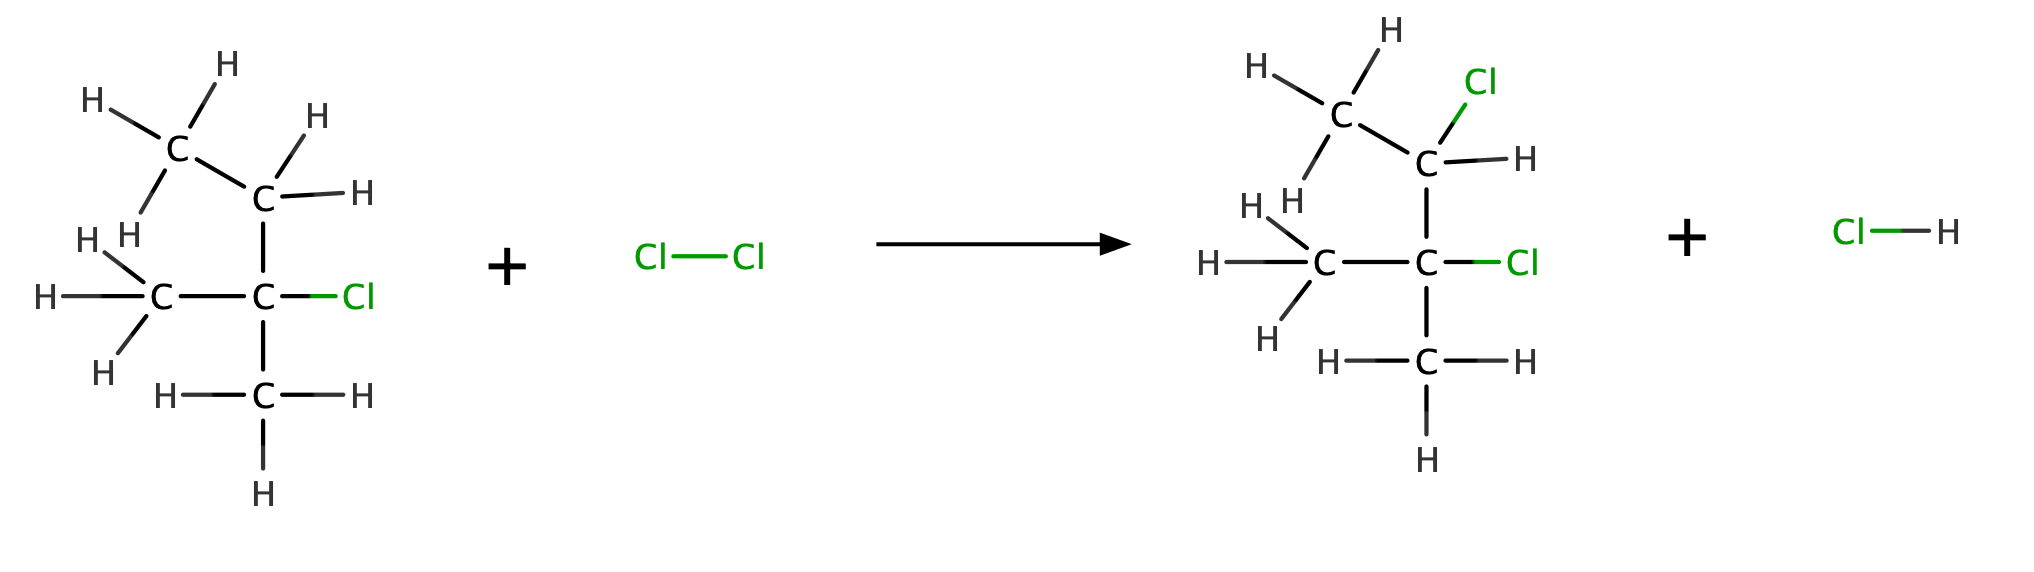
\includegraphics[scale=0.4]{O2_4.png}
\end{center}
\caption{Reaktionsskema lavet vha. MarvinSketch}
\label{fig:4}
\end{figure}
\textbf{c.} Reaktionsskemaet ses i \cref{fig:5}, hvor reaktionsproduktet hedder 2,3-dibrom-3-methylpentan. Bemærk dog, at der kan være Z,E-isomeri med hensyn til 3-methylpent-2-en.
\begin{figure}[H]
\begin{center}
  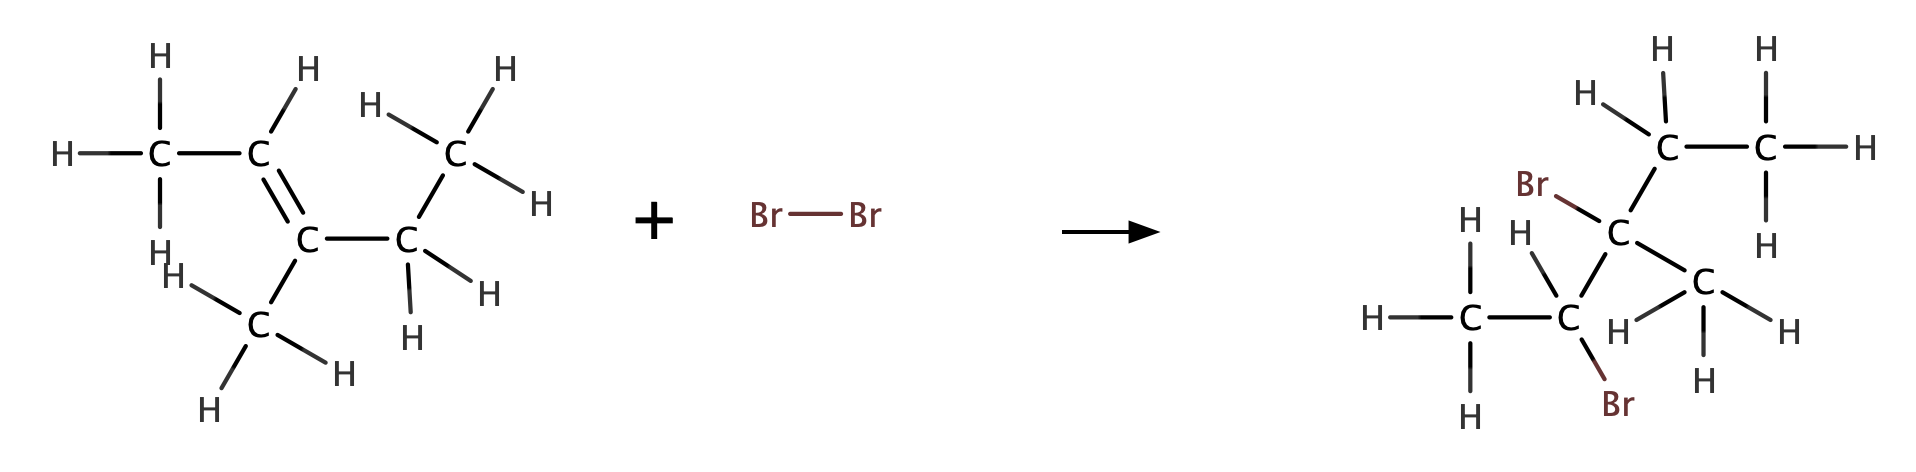
\includegraphics[scale=0.4]{O2_5.png}
\end{center}
\caption{Reaktionsskema lavet vha. MarvinSketch}
\label{fig:5}
\end{figure}
\textbf{d.} Reaktionen følger Markovnikovs regel. Så vil chlor-atomet binde sig til det sekundære carbonatom, hvor hydrogenatomet vil binde sig til det primære. Reaktionsskemaet ses i \cref{fig:7}, hvor reaktionsproduktet hedder 2-chlorheptan.
\begin{figure}[H]
\begin{center}
  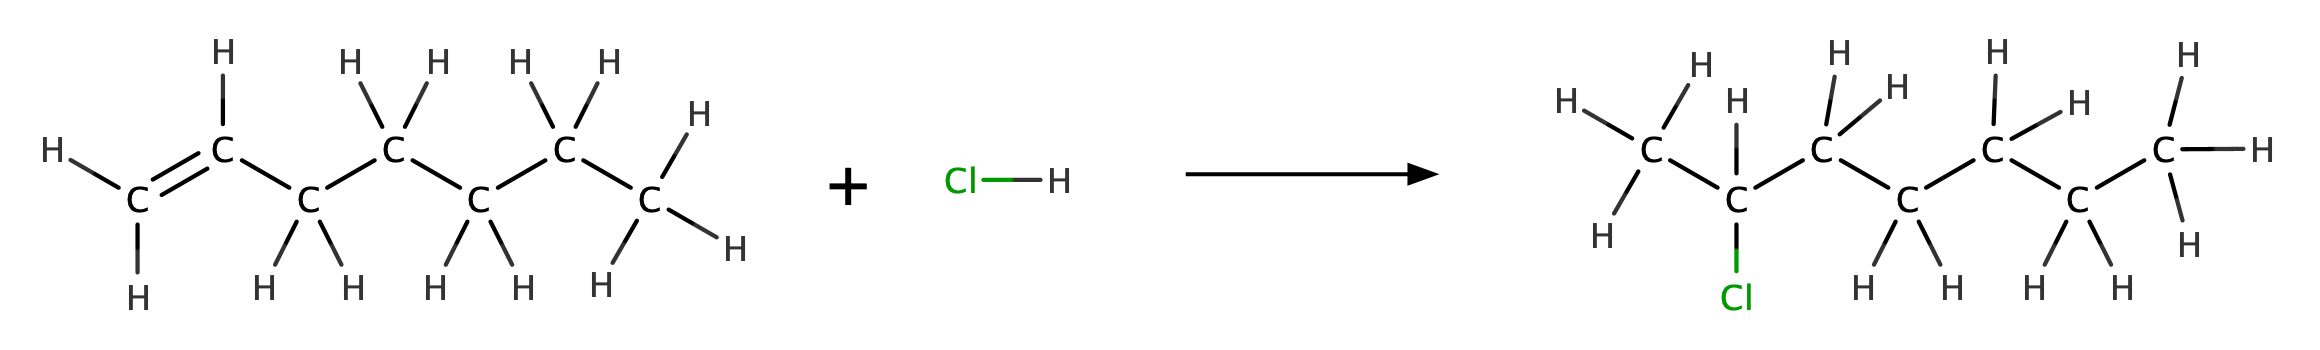
\includegraphics[scale=0.4]{O2_7.png}
\end{center}
\caption{Addition af hydrogenchlorid til hept-1-en}
\label{fig:7}
\end{figure} 
\textbf{e.} Et eksempel på et reaktionsskema er givet i \cref{fig:8}, hvor reaktionsprodukterne er hex-1-en og dihydrogenoxid. I stedet for hex-1-en kan det også være \textit{cis}-hex-2-en og \textit{trans}-hex-2-en.
\begin{figure}[H]
\begin{center}
  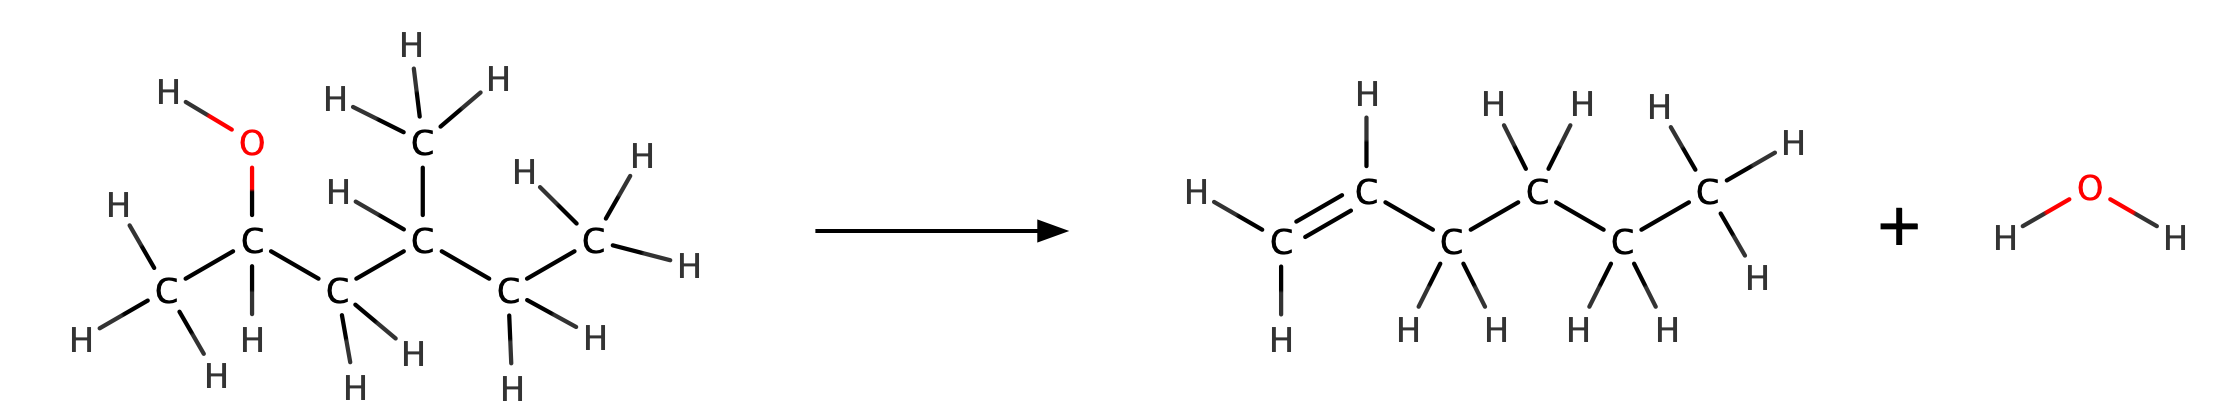
\includegraphics[scale=0.4]{O2_8.png}
\end{center}
\caption{Elimination af vand fra 4-methylhexan-2-ol}
\label{fig:8}
\end{figure}

\section*{Opgave 2.15}
\sol \\
\textbf{a.} 
Det systematiske navn for $\text{SmartFresh}^{\text{SM}}$ er da 1-methylcycloprop-1-en. \\[1ex]
\textbf{b.} Reaktionsprodukterne for de tre anførte additionsreaktioner kan ses i \cref{fig:9}, hvor Markovnikovs regel igen er brugt.
\begin{figure}[H]
\begin{center}
  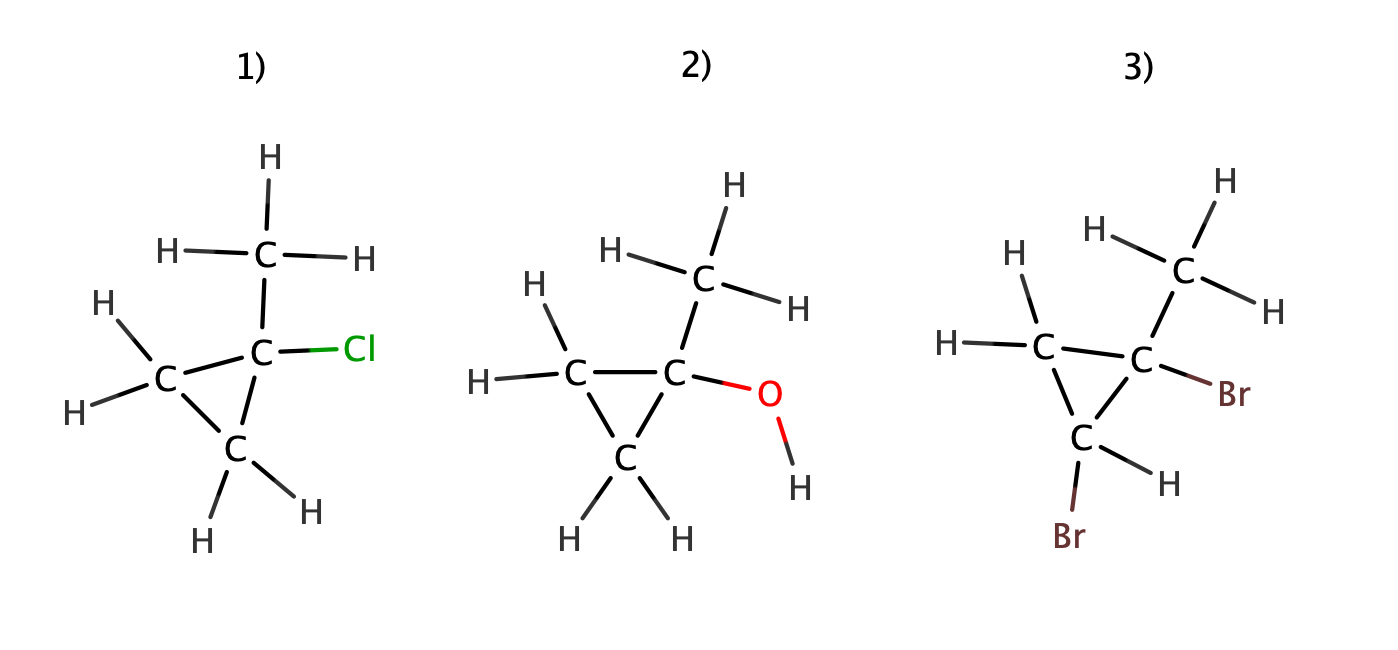
\includegraphics[scale=0.4]{O2_9.png}
\end{center}
\caption{Reaktionsprodukterne for de tre anførte additionsreaktioner}
\label{fig:9}
\end{figure}

\end{document}
